
\section{Agents - Terminal, Pilot, and Child}
\label{sec:agents}

All\marginnote{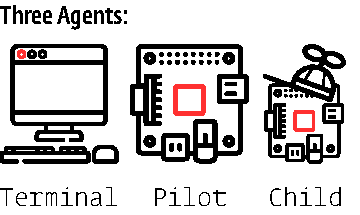
\includegraphics[]{figures/side_26_agents.pdf}} of the above components---tasks, hardware, and stimuli---are organized into a single system as an "agent," the central executable component of Autopilot which a) manages the core operations of the system and b) defines how it interacts with the rest of the agents it is connected to. Specifically, agents are built around an action vocabulary that  maps different types of messages to callback methods.

\clearpage

Currently, we have implemented three Agent types: 

\begin{itemize}
    \item \textbf{Terminal} - The user-facing control agent.
    \item \textbf{Pilot} - A Raspberry Pi that runs tasks, coordinates hardware, and optionally coordinates a set of child Pis.
    \item \textbf{Child} - Subordinate Pis to a pilot that carry out different parts of a task
\end{itemize}

\textbf{Terminal}\marginnote{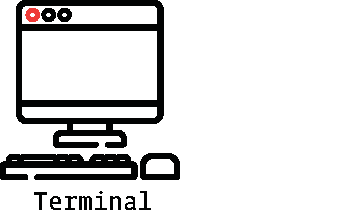
\includegraphics[]{figures/side_27_terminal.pdf}} agents serve as a root node (see Section \ref{sec:networking}) in an Autopilot swarm. The terminal is the only agent with a \hyperref[sec:ui]{GUI}, which is used to control its connected pilots and visualize incoming task data. The terminal also manages data and keeps a registry of all active experimental subjects. The terminal is intended to make the day-to-day use of an Autopilot swarm manageable, even for those without programming experience. The terminal GUI is described further in Section \ref{sec:ui}.

\textbf{Pilot}\marginnote{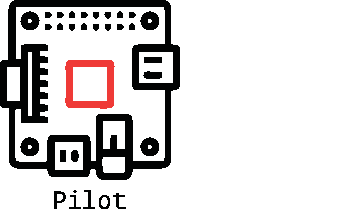
\includegraphics[]{figures/side_28_pilot.pdf}} agents are the workhorses of Autopilot---the agents that run the experiments. Pilots are intended to operate as always-on, continuously running system services. Pilots make a network connection to a terminal and wait for further instructions. They maintain the system-level software used for interfacing with the hardware connected to the Raspberry Pi, receive and execute tasks, and continually return data to the terminal for storage. 

Each\marginnote{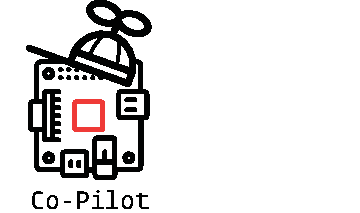
\includegraphics[]{figures/side_29_child.pdf}} pilot is capable of coordinating one or many \textbf{child} agents. The pilot maintains a network connection to its children, and if a task specifies that some of its functionality is to be split between Raspberry Pis, the pilot notifies its children and sends them a specialized subtask description. The pilot serves as the only point of contact between its children and the terminal, so the terminal only needs to keep track of its pilots, and doesn't need separate methods for communicating with all their children, their hardware, etc.

\subsection{Behavioral topologies}
\label{sec:topology}

We think one of the most transformative features of Autopilot's distributed structure is the control that users have over what we call "behavioral topology." The logic of hardware and task operation within an agent, the distribution of labor between agents performing a task, and the pattern of connectivity and command within a swarm of agents constitute a topology. 

Below we illustrate this idea with a few examples:

\clearpage

\begin{itemize}
    \item \textbf{Pilot Swarm}\marginnote{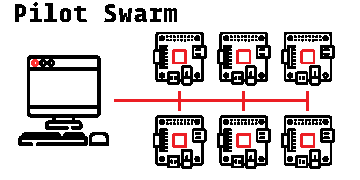
\includegraphics[]{figures/side_20_swarm.pdf}} - The first and most obvious topological departure from traditional behavioral instrumentation is the use of a single computer to independently coordinate tasks in parallel. Our primary installation of Autopilot is a cluster of 10 behavior boxes that can independently run tasks dispatched from a central terminal which manages data and visualization. This topology highlights the expandability of an Autopilot system: adding new pilots is inexpensive, and the single central terminal makes controlling experiments and managing data simple.
    \item \textbf{Shared Task} - \marginnote{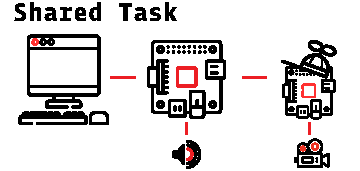
\includegraphics[]{figures/side_21_shared.pdf}} Tasks can be shared across pilots and their (potentially multiple) children to handle tasks with computationally intensive operations. For example, in an open-field navigation task, one pilot can deliver position-dependent sounds while one of its children records and analyzes video of the arena to track the animal's position. The terminal only needs to be configured to connect to the parent pilot, but since networking is handled in an independent process the raw video data can pass through the parent from the child such that sound delivery remains responsive.
    \item \textbf{Distributed Task}\marginnote{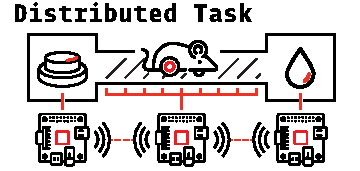
\includegraphics[]{figures/side_22_distributed.pdf}} - Many pilots with overlapping responsibilities can cooperate to perform distributed tasks. We anticipate this will be useful when the experimental arenas can't be fully contained (such as natural environments), or when experiments require simultaneous input and output from multiple subjects. Distributed tasks can take advantage of the Pi's wireless communication, enabling, for example, experiments that require many networked cameras to observe an area, or experiments that use the Pis themselves as an interface in a multisubject augmented reality experiment.
    \item \textbf{Multi-Agent Task}\marginnote{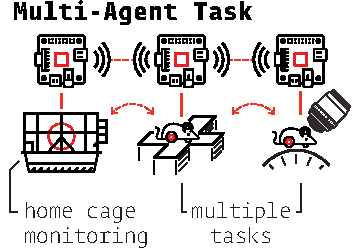
\includegraphics[]{figures/side_23_multi.pdf}} - Neuroscientific research often consists of multiple mutually interdependent experiments, each with radically different instrumentation. Autopilot provides a framework to unify these experiments by allowing users to rewrite core functionality of the program while maintaining integration between its components. For example, a neuroethologist could build a new \hyperref[sec:futureagents]{"Observer"} agent that continually monitors an animal's natural behavior in its home cage to calibrate a parameter in a task run by a pilot. If they wanted to manipulate the behavior, they could build a "Compute" agent that processes Calcium imaging data taken while the animal performs the task to generate and administer patterns of optogenetic stimulation. We think that unifying diverse experimental data streams and hardware into a single framework is the best way to perform experiments that measure natural behavior and its hierarchical organization across multiple timescales in order to  understand the naturally behaving brain\citep{dattaComputationalNeuroethologyCall2019}.
\end{itemize}
